\documentclass[12pt]{article}
\usepackage{tikz}
\usepackage{amsmath}
\usepackage{amssymb}
\usepackage{graphicx}
\usepackage{subcaption}
\usepackage{booktabs}
\usepackage[margin=1in]{geometry}

\title{Intuitive Explanation of Physics-Informed Neural Networks (PINNs)}
\author{For Finite Element Experts}
\date{}

\begin{document}

\maketitle

\section*{Core Concept: PINNs as Constrained Optimizers}
PINNs train neural networks to satisfy:
\begin{itemize}
    \item Governing PDE equations
    \item Boundary conditions (BCs)
    \item Initial conditions (ICs)
\end{itemize}
through a \textbf{composite loss function}. The network learns by minimizing violations of these physical constraints.

\section*{Key Components of PINN Loss Function}
The total loss ($\mathcal{L}_{\text{total}}$) combines multiple constraint violations:

\begin{equation}
\mathcal{L}_{\text{total}} = \underbrace{w_{\text{PDE}} \mathcal{L}_{\text{PDE}}}_{\text{PDE residual}} + 
\underbrace{w_{\text{BC}} \mathcal{L}_{\text{BC}}}_{\text{Boundary violation}} + 
\underbrace{w_{\text{IC}} \mathcal{L}_{\text{IC}}}_{\text{Initial condition}}
\end{equation}

\subsection*{1. PDE Loss ($\mathcal{L}_{\text{PDE}}$)}
Measures how well the solution satisfies the governing PDE at \textit{collocation points} inside the domain:

\begin{equation}
\mathcal{L}_{\text{PDE}} = \frac{1}{N_{\text{PDE}}} \sum_{i=1}^{N_{\text{PDE}}} \left\| \mathcal{N}[u_{\theta}(\mathbf{x}_i)] - f(\mathbf{x}_i) \right\|^2
\end{equation}

\begin{itemize}
    \item $\mathcal{N}$: Differential operator (e.g., $\nabla^2$, $\frac{\partial}{\partial t}$)
    \item $u_{\theta}$: NN prediction with parameters $\theta$
    \item $f$: Source term
    \item Derivatives computed via \textbf{automatic differentiation}
\end{itemize}

\subsection*{2. Boundary Condition Loss ($\mathcal{L}_{\text{BC}}$)}
Enforces boundary constraints at sampled boundary points:

\begin{equation}
\mathcal{L}_{\text{BC}} = \frac{1}{N_{\text{BC}}} \sum_{j=1}^{N_{\text{BC}}} \left\| B[u_{\theta}(\mathbf{x}_j)] - g(\mathbf{x}_j) \right\|^2
\end{equation}

\begin{itemize}
    \item $B$: Boundary operator (Dirichlet, Neumann, etc.)
    \item $g$: Prescribed boundary value
\end{itemize}

\subsection*{3. Initial Condition Loss ($\mathcal{L}_{\text{IC}}$)}
For time-dependent problems, enforces initial state:

\begin{equation}
\mathcal{L}_{\text{IC}} = \frac{1}{N_{\text{IC}}} \sum_{k=1}^{N_{\text{IC}}} \left\| u_{\theta}(\mathbf{x}_k, t=0) - h(\mathbf{x}_k) \right\|^2
\end{equation}

\begin{figure}[h]
    \centering
    \includegraphics[width=0.8\textwidth]{fig.png}
    \caption{PINN architecture showing loss components}
    \label{fig:pinn}
\end{figure}

\section*{Critical Insight: Soft vs. Hard Constraints}
\begin{table}[h]
    \centering
    \begin{tabular}{p{6cm}p{6cm}}
        \toprule
        \textbf{Soft Constraints (Standard PINNs)} & \textbf{Hard Constraints} \\
        \midrule
        Constraints enforced via loss terms & Constraints \textit{built into} network architecture \\
        BCs/ICs appear as penalty terms & BCs/ICs are \textit{exactly satisfied} by construction \\
        $u_{\theta}$ can violate constraints during training & No constraint violation possible \\
        Weights ($w_{\text{BC}}$, $w_{\text{IC}}$) require tuning & No weighting needed \\
        Easier to implement & Requires specialized architecture \\
        \bottomrule
    \end{tabular}
    \caption{Constraint implementation strategies}
\end{table}

\section*{Why Derivatives Work in PINNs}
\begin{itemize}
    \item \textbf{Automatic differentiation} computes \textit{exact derivatives} of $u_{\theta}$ (not finite differences)
    \item PDE loss directly compares NN's derivatives to physical laws
    \item Gradient descent propagates PDE violation errors backward through:
    \begin{equation}
    \frac{\partial \mathcal{L}_{\text{PDE}}}{\partial \theta} = \frac{2}{N} \sum \left(\mathcal{N}[u_{\theta}] - f\right) \cdot \frac{\partial \mathcal{N}[u_{\theta}]}{\partial \theta}
    \end{equation}
    \item The NN \textbf{simultaneously} learns function values \textit{and} derivatives
\end{itemize}

\section*{Training Dynamics Visualization}
\begin{center}
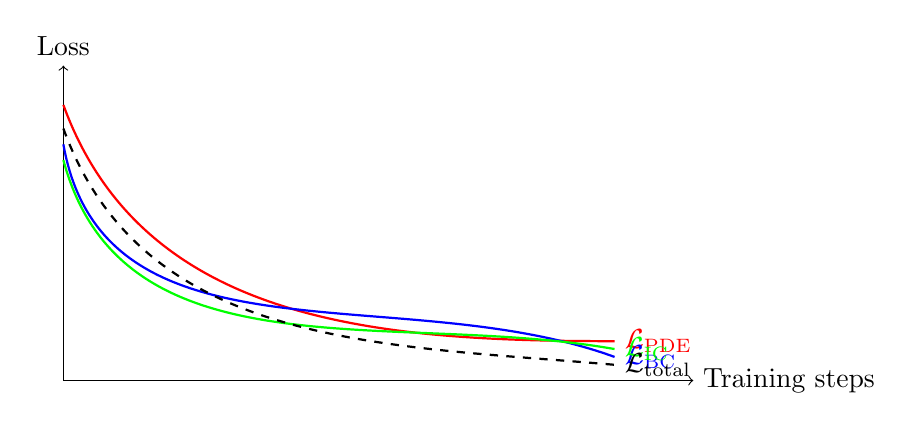
\begin{tikzpicture}
    \draw[->] (0,0) -- (8,0) node[right] {Training steps};
    \draw[->] (0,0) -- (0,4) node[above] {Loss};
    \draw[red, thick] (0,3.5) to[out=-70, in=180] (7,0.5) node[right] {$\mathcal{L}_{\text{PDE}}$};
    \draw[blue, thick] (0,3) to[out=-80, in=160] (7,0.3) node[right] {$\mathcal{L}_{\text{BC}}$};
    \draw[green, thick] (0,2.8) to[out=-75, in=170] (7,0.4) node[right] {$\mathcal{L}_{\text{IC}}$};
    \draw[black, dashed, thick] (0,3.2) to[out=-70, in=175] (7,0.2) node[right] {$\mathcal{L}_{\text{total}}$};
\end{tikzpicture}
\end{center}

\section*{Key Advantages for FEM Experts}
\begin{itemize}
    \item \textbf{No meshing}: Collocation points can be randomly sampled
    \item \textbf{Unified framework}: Handles both forward and inverse problems
    \item \textbf{Adaptive refinement}: Loss guides where to add collocation points
    \item \textbf{High-dimensional problems}: Avoids curse of dimensionality
\end{itemize}

\section*{Conclusion: Loss as Physics Interpreter}
The PINN loss function acts as a \textit{physics interpreter} that:
\begin{enumerate}
    \item Translates PDEs into optimization constraints
    \item Quantifies violations of physical laws
    \item Balances multiple constraints through weighting
    \item Provides training signals via automatic differentiation
\end{enumerate}
The network becomes a \textbf{continuous function approximator} that satisfies physics in the weak sense defined by the composite loss.

\end{document}